
\documentclass[9pt]{beamer}
%\makeatletter
%\def\beamer@calltheme#1#2#3{%
%	\def\beamer@themelist{#2}
%	\@for\beamer@themename:=\beamer@themelist\do
%	{\usepackage[{#1}]{\beamer@themelocation/#3\beamer@themename}}}
%
%\def\usefolder#1{
%	\def\beamer@themelocation{#1}
%}
%\def\beamer@themelocation{}

%\usefolder{../config}

\usetheme[
block=fill,
titleformat=regular,
progressbar=frametitle
]{metropolis}
%\metroset[everytitleformat=regular] % regular, lowercase, uppercase ]
%\metroset[inner/block=fill]

%\setbeameroption{show notes} 
\usepackage{booktabs}
\usepackage[scale=2]{ccicons}

\usepackage{pgfplots}
\usepgfplotslibrary{dateplot}


%\ Hrvatski znakovi
\usepackage[utf8]{inputenc}
\usepackage[T1]{fontenc}
\usepackage[croatian]{babel}
\usepackage{todonotes}
\usepackage{amsmath}
\usepackage{amsfonts}
\selectlanguage{croatian} % american ngerman
\usepackage{todonotes}

% Koristenje Latin modern fonta
% Bez toga na nekim racunalima baca
% err: Font <taj i taj> at <mala velicina, npr4.0pt> not loadable: Metric (TFM) file not found. \end{frame}
\usepackage{lmodern}


\definecolor{RoyalBlue}{cmyk}{1, 0.50, 0, 0}
%\usepackage{natbib}
%\usepackage{bibentry}
\usepackage{scrextend}
\usepackage{hyperref}
%\usepackage[pdfa=true]{hyperref}
\hypersetup{%
    %draft, % = no hyperlinking at all (useful in b/w printouts)
    %colorlinks=true, 
    linktocpage=true, pdfstartpage=3, pdfstartview=FitV,%
    % uncomment the following line if you want to have black links (e.g., for printing)
    %colorlinks=false, linktocpage=false, pdfborder={0 0 0}, pdfstartpage=3, pdfstartview=FitV,% 
    breaklinks=true, pdfpagemode=UseNone, pageanchor=true, pdfpagemode=UseOutlines,%
    plainpages=false, bookmarksnumbered, bookmarksopen=true, bookmarksopenlevel=1,%
    hypertexnames=true, pdfhighlight=/O,%nesting=true,%frenchlinks,%
    %urlcolor=webbrown, linkcolor=RoyalBlue, citecolor=webgreen, %pagecolor=RoyalBlue,%
    %urlcolor=Blue, linkcolor=Blue, citecolor=Red, %pagecolor=Black,%
    %pdftitle={\myTitle},%
    %pdfauthor={\textcopyright\ \myName, \myUni, \myFaculty},%
    pdfsubject={},%
    pdfkeywords={},%
    pdfcreator={pdfLaTeX},%
    pdfproducer={LaTeX with hyperref and classicthesis}, %
    unicode = true 
} 

%\usepackage[pdftex]{graphicx}
% declare the path(s) where your graphic files are
\graphicspath{{./}{./figures/}}


\newcommand{\executeiffilenewer}[3]{%
	\ifnum\pdfstrcmp{\pdffilemoddate{#1}}%
	{\pdffilemoddate{#2}}>0%
	{\immediate\write18{#3}}\fi%
}
\newcommand{\includesvg}[1]{%
	\executeiffilenewer{#1.svg}{#1.pdf}%
	{inkscape -z -C --file=#1.svg %
		--export-pdf=#1.pdf --export-latex}%
	\input{#1.pdf_tex}%
}


% http://tex.stackexchange.com/questions/83882/how-to-highlight-python-syntax-in-latex-listings-lstinputlistings-command

\usepackage{listings}
\usepackage{color}
\usepackage[semibold]{sourcecodepro}

% Default fixed font does not support bold face
\DeclareFixedFont{\ttb}{T1}{txtt}{bx}{n}{12} % for bold
\DeclareFixedFont{\ttm}{T1}{txtt}{m}{n}{12}  % for normal
% Custom colors
\definecolor{deepblue}{rgb}{0,0,0.5}
\definecolor{deepred}{rgb}{0.6,0,0}
\definecolor{deepgreen}{rgb}{0,0.5,0}


% Python style for highlighting
\newcommand\pythonstyle{\lstset{
		language=Python,
		basicstyle=\small\ttfamily,
		otherkeywords={self},             % Add keywords here
		keywordstyle=\small\ttfamily\color{deepblue},
		emph={MyClass,__init__},          % Custom highlighting
		emphstyle=\small\ttfamily\color{deepred},    % Custom highlighting style
		stringstyle=\color{deepgreen},
		frame=tb,                         % Any extra options here
		showstringspaces=false            % 
	}}
	
	
	% Python environment
	\lstnewenvironment{python}[1][]
	{
		\pythonstyle
		\lstset{#1}
	}
	{}
	
	% Python for external files
	\newcommand\pythonexternal[2][]{{
			\pythonstyle
			\lstinputlisting[#1]{#2}}}
	
	% Python for inline
	\newcommand\pythoninline[1]{{\pythonstyle\lstinline!#1!}}

% \includeonlyframes{current}

%\documentclass[ucs]{beamer}
%\usetheme[menuwidth={0.3\paperwidth}]{erlangen}
%\setbeamercovered{transparent=20} 

\usepackage{amsmath,amsfonts,amsthm,amssymb}
\usepackage{setspace}
\usepackage{Tabbing}
\usepackage{fancyhdr}
\usepackage{lastpage}
\usepackage{extramarks}
\usepackage{chngpage}
\usepackage{soul,color}
\usepackage{graphicx,float,wrapfig}
\usepackage{xcolor}
\usepackage[normalem]{ulem}
\usepackage{mathtools}

\definecolor{erlangenlyellow}{RGB}{123, 25, 121}
%\usepackage[utf8x]{inputenc}
%\usepackage{default}
%\usepackage[T1]{fontenc}

\usepackage{verbatim}
\usepackage{listings}


\usepackage{subcaption}
\usepackage{lmodern}

\title{Transformacije}

\subtitle{ I might find balance $\ldots$ But I won't}
\institute{Računalna grafika}


\begin{document}
\begin{frame}
 \titlepage
\end{frame}

%\begin{frame}{Sadržaj}
%  \tableofcontents
%  % You might wish to add the option [pausesections]
%\end{frame}
\section{Klasifikacija transformacija}

\begin{frame}{Umjesto definicije}
	Funkcija koja preslikava točku $x$ u $x'$
	\begin{center}
		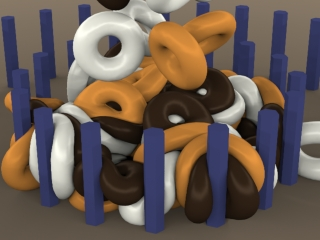
\includegraphics[height=3cm]{slike/tori.png}
		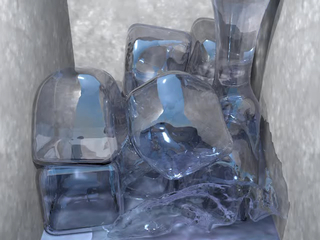
\includegraphics[height=3cm]{slike/ice_stacked.png}
	\end{center}
\end{frame}
% % % % % % % % % % % % % % % % % % % % % % % % % % % % % % % % % % % % % % % % % % % % % %
\begin{frame}{Jednostavne transformacije}
	\begin{figure}
		\begin{center}
			\begin{subfigure}[b]{0.35\linewidth}
				
\includegraphics[height=3cm]{slike/funny_cow_template_1.png}
				\caption{Identitet}
			\end{subfigure}
			\begin{subfigure}[b]{0.35\linewidth}
				
\includegraphics[height=3cm]{slike/funny_cow_translate.png}
				\caption{Translacija}
			\end{subfigure}
			\begin{subfigure}[b]{0.35\linewidth}
				
\includegraphics[height=3cm]{slike/funny_cow_rotate.png}
				\caption{Rotacija}
			\end{subfigure}
			\begin{subfigure}[b]{0.35\linewidth}
				
\includegraphics[height=3cm]{slike/funny_cow_scale.png}
				\caption{Uniformno skaliranje}
			\end{subfigure}
		\end{center}
	\end{figure}
\end{frame}

\begin{frame}{Euklidske transformacije}
	Ili transformacije krutog tijela.
	\begin{itemize}
		\item Očuvane udaljenosti
		\item Očuvani kutevi
	\end{itemize}
	\begin{figure}
		\begin{subfigure}[b]{0.35\linewidth}
			
\includegraphics[height=3cm]{slike/funny_cow_translate.png}
			\caption{Translacija}
		\end{subfigure}
		\begin{subfigure}[b]{0.35\linewidth}
			
\includegraphics[height=3cm]{slike/funny_cow_rotate.png}
			\caption{Rotacija}
		\end{subfigure}
	\end{figure}
\end{frame}

\begin{frame}{Sličnost}
	Ovdje spada sve prije + izotropno skaliranje
	\begin{itemize}
		\item Očuvani kutevi
		\item Oblik je isti, ali s različitom skalom, orijentacijom i pozicijom
		
	\end{itemize}
\end{frame}

\begin{frame}{Linearne transformacije}
	\begin{figure}
		\begin{center}
			\begin{subfigure}[b]{0.3\linewidth}
				
\includegraphics[height=1.8cm]{slike/funny_cow_scale_2.png}
				\caption{Skaliranje}
			\end{subfigure}
			\begin{subfigure}[b]{0.3\linewidth}
				
\includegraphics[height=1.8cm]{slike/funny_cow_mirror.png}
				\caption{Zrcaljenje}
			\end{subfigure}
			\begin{subfigure}[b]{0.3\linewidth}
				
\includegraphics[height=1.8cm]{slike/funny_cow_shear.png}
				\caption{Smik}
			\end{subfigure}
		\end{center}
	\end{figure}
	Grafička interpretacija: transformacija točaka oko (u odnosu na) ishodišta.\\
	Pod linearne transformacije spada sve navedeno osim translacije, odnosno vrijedi:
	\begin{itemize}
		\item $f(\mathbf{p}+\mathbf{q}) = f(\mathbf{p}) + f(\mathbf{q})$
		\item $f(a\mathbf{q}) = af(\mathbf{p})$
	\end{itemize}
\end{frame}


\begin{frame}{Linearne transformacije contd.}
	\begin{Large}
		\textbf{Translacija NIJE linearna!}
	\end{Large}
	\begin{itemize}
		\item $f(p) = p+t$
		\item $f(ap) = ap+t \neq a(p+t) = af(p)$
		\item $f(p+q) = p+q+t \neq (p+t)+(q+t) = f(p)+f(q)$
	\end{itemize}
\end{frame}

\begin{frame}{Afine transformacije}
	Linearne transformacije + translacija.\\
	Ostaju očuvane paralelne linije
	\begin{figure}
		
\includegraphics[height=3cm]{slike/funny_cow_complex_transform.png}
	\end{figure} 
\end{frame}

\begin{frame}{Perspektivne transformacije}
	Očuvane su linije
	\begin{figure}
		
\includegraphics[height=3cm]{slike/funny_cow_perspective.png}
	\end{figure}
\end{frame}

\begin{frame}{Transformacije u slici}
	\begin{figure}
		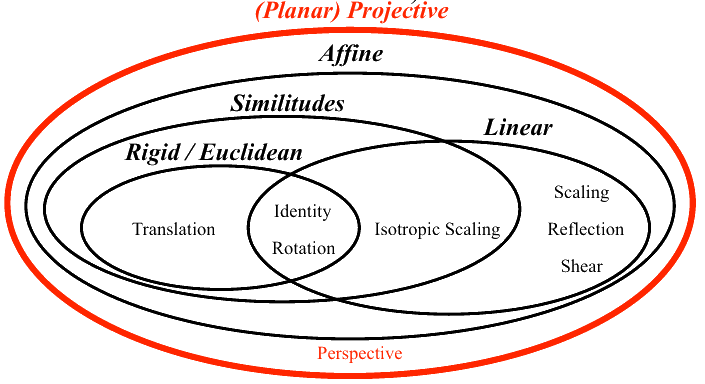
\includegraphics[width=10cm]{slike/tansformacije_tipovi.png}
	\end{figure}
\end{frame}

\begin{frame}{Posljedica hijerarhije}
	\begin{block}{Korist}
		Zatvorenost: Rezultat dvije afine transformacije jest afina transformacija
	\end{block}
	Vrijedi za svaku grupu i podgrupu transformacija
	\begin{block}{Iznimno mudro\ldots}
			Skup $S$ definiran operacijom\footnote[frame]{binarnom operacijom, da budemo precizniji} $f$ na skupu $S$, gdje je svako preslikavanje element skupa $S$, jest grupa.\\
			$s,t \in S$, $f(s,t) = u \Rightarrow u \in S$ itd.\\
			Transformacije su grupe i podgrupe. Odnosno transformacije su $S$, dok je ulančavanje transformacija $f$.
	\end{block}
\end{frame}

\begin{frame}{Transformacije su grupe. I?}
	\textbf{Moguće je prikazati bilo koji broj sukcesivnih transformacija s jednom općom transformacijom}
\end{frame}

\section{Transformacije i matrice}

\begin{frame}{Linearne transformacije}
	\begin{itemize}
		\item Linearne transformacije se obično provode s invertibilnim matricama% \footnote[frame]{hey candy cane brain pouring like the rain}
		\item 2D transformacija : 
	\end{itemize}
	\begin{align*}
		\mathbf{T}= \left [ \begin{array}{cc}
		a & b  \\
		c & d  \end{array} \right]
	\end{align*}
	\begin{itemize}
		\item Transformacija vektora $\mathbf{x}$
	\end{itemize}
	\begin{align*}
		\left[ \begin{array}{c} x_{1} \\ x_{2}  \end{array} \right] \rightarrow 
		\left[ \begin{array}{cc}
		a & b  \\
		c & d  \end{array} \right] 	\left[ \begin{array}{c} x_{1} \\ x_{2}    \end{array} \right] = 
		\left[ \begin{array}{c}
		ax_{1} + bx_{2}  \\
		cx_{1} + dx_{2}  \end{array} \right]\nonumber
		\end{align*}
\end{frame}

\begin{frame}{Linearne transformacije}
	\begin{center}
		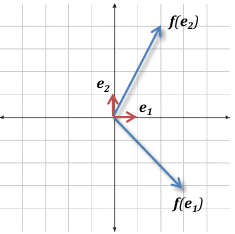
\includegraphics[height=2cm]{slike/basis_vector.png}
	\end{center}
	
		\begin{align*}
		\mathbf{e}_{1} = \left[ \begin{array}{c} 1 \\ 0  \end{array} \right]\ 
		\mathbf{e}_{2} = \left[ \begin{array}{c} 0 \\ 1  \end{array} \right]
		\nonumber
		\end{align*}
	
		\begin{align*}
		T \left[ \begin{array}{c} 1 \\ 0  \end{array} \right]\ =
		\left[ \begin{array}{cc}
		a & b  \\
		c & d  \end{array} \right] \left[ \begin{array}{c} 1 \\ 0  \end{array} \right] = 
		\left[ \begin{array}{c} a \\ c  \end{array} \right] \Rightarrow
		\mathbf{T}_{1}(\mathbf{e}_{1}) = \left[ \begin{array}{c} a \\ c  \end{array} \right]
		\nonumber
		\end{align*}
		\begin{align*}
		T \left[ \begin{array}{c} 0 \\ 1  \end{array} \right]\ =
		\left[ \begin{array}{cc}
		a & b  \\
		c & d  \end{array} \right] \left[ \begin{array}{c} 0 \\ 1  \end{array} \right] = 
		\left[ \begin{array}{c} b \\ d  \end{array} \right] \Rightarrow
		\mathbf{T}_{2}(\mathbf{e}_{2}) = \left[ \begin{array}{c} b \\ d  \end{array} \right]
		\nonumber
		\end{align*}
	
\end{frame}
\begin{frame}{Linearne transformacije  - Rotacija}
	\begin{center}
		
\includegraphics[height=1.5cm]{slike/funny_cow_rotate.png} \\
		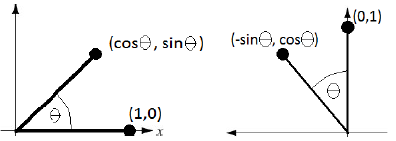
\includegraphics[height=1.5cm]{slike/basis_vector_rotation.png}
	\end{center}
	Rotacija za kut $\theta$ oko ishodišta - $\mathbf{v}' = \mathbf{R}\mathbf{v}$
	
		\begin{align*}
		e_{1} \left[ \begin{array}{c} 1 \\ 0  \end{array} \right] \Rightarrow
		\left[ \begin{array}{c} \cos\theta \\ \sin \theta  \end{array} \right]
		\qquad\qquad
		e_{2} \left[ \begin{array}{c} 0 \\ 1  \end{array} \right] \Rightarrow
		\left[ \begin{array}{c} -\sin\theta \\ \cos\theta  \end{array} \right]  
		\end{align*}
		\begin{align*}
		\mathbf{R} =  \left[ \begin{array}{cc} \mathrm{cos}\theta & -\sin\theta \\ 
		\sin\theta & \cos\theta  \end{array} \right]
		\nonumber
		\end{align*}
\end{frame}

\begin{frame}{Linearne transformacije  - Rotacija contd.}
	\begin{center}
		
\includegraphics[height=1.5cm]{slike/funny_cow_rotate.png}
	\end{center}
	
		\begin{align*}
		\mathbf{R} \mathbf{v}=  \left[ \begin{array}{cc} \cos\theta & -\sin\theta \\ 
		\sin\theta & \cos\theta  \end{array} \right] 
		\left[ \begin{array}{c} x \\ y  \end{array} \right] = 
		\left[ \begin{array}{c} x \cos\theta - y  \sin\theta\\ 
		x \sin\theta + y  \cos\theta  \end{array} \right]
		\end{align*}
	Rotacija UVIJEK oko ishodišta
	\begin{block}{Linearne tranformacije, podsjetnik}
			Linearne transformacije uključuju rotaciju, skaliranje, zrcaljenje i smik.
			Ishodište je fiksno
		\end{block}
	
\end{frame}

\begin{frame}{Linearne transformacije  - Skaliranje}
	$$s_{x} =3, s_{y} = 2$$
	
		\begin{equation}
		\mathbf{s} =  \left[ \begin{array}{c} s_{x} \\ s_{y}  \end{array} \right]
		\nonumber
		\end{equation}
	$$\mathbf{v}' = \mathbf{s}\mathbf{v}$$
	
		\begin{equation}
		e_{1} \left[ \begin{array}{c} 1 \\ 0  \end{array} \right] \Rightarrow
		s_{x}e_{1} = \left[ \begin{array}{c} s_{x} \\ 0  \end{array} \right] 
		\nonumber
		\end{equation}
	
	
		\begin{equation}
		e_{2} \left[ \begin{array}{c} 0 \\ 1  \end{array} \right] \Rightarrow
		s_{y}e_{2} = \left[ \begin{array}{c} 0 \\ s_{y}  \end{array} \right] 
		\nonumber
		\end{equation}
	
	
		\begin{equation}
		\mathbf{S} =  \left[ \begin{array}{cc} s_{x} & 0 \\ 0 & s_{y}  \end{array} \right] \Rightarrow
		\mathbf{S}\mathbf{v} = \left[ \begin{array}{cc} s_{x} & 0 \\ 0 & s_{y}  \end{array} \right]
		\left[ \begin{array}{c} x \\ y  \end{array} \right] = 
		\left[ \begin{array}{c} s_{x}x \\ s_{y}y  \end{array} \right] 
		\nonumber
		\end{equation}
\end{frame}

\begin{frame}{Zrcaljenje}
	\begin{center}
		
\includegraphics[height=1.cm]{slike/funny_cow_mirror.png}
	\end{center}
	Oko $y$ osi:
	\begin{equation}
	\mathbf{M}\mathbf{v} = \left[ \begin{array}{cc} -1 & 0 \\ 
	0 & 1  \end{array} \right] 
	\left[ \begin{array}{c} x \\ y  \end{array} \right] = 
	\left[ \begin{array}{c} -x  \\ 
	y  \end{array} \right]
	\nonumber
	\end{equation}
	
	Oko $x$ osi:
	\begin{equation}
	\mathbf{M}\mathbf{v} = \left[ \begin{array}{cc} 1 & 0 \\ 
	0 & -1  \end{array} \right] 
	\left[ \begin{array}{c} x \\ y  \end{array} \right] = 
	\left[ \begin{array}{c} x  \\ 
	-y  \end{array} \right]
	\nonumber
	\end{equation}
	
\end{frame}

\begin{frame}{Intermezzo}
	\begin{block}{Blago zanimljivo}
		Matrica rotacije i zrcaljenja je ortogonalna 
	\end{block}
	\begin{block}{Ortogonalna matrica}
		$$\mathbf{M}^{-1} = \mathbf{M}^T$$
	\end{block}
	\begin{block}{Zanimljiva svojstva}
		Ortogonalna matrica $\mathbf{M}$ će očuvati duljinu, odnosno:
		$$||\mathbf{M}\mathbf{P}|| = ||\mathbf{P}||$$
		Također, očuvat će i kuteve:
		$$(\mathbf{M}\mathbf{P}_1) (\mathbf{M}\mathbf{P}_2)= \mathbf{P}_1\mathbf{P}_2$$
	\end{block}
\end{frame}

\begin{frame}{Afine transformacije}
	\begin{eqnarray}\nonumber
	x' = ax+by + c \\
	y' = dx+ey + f\nonumber
	\end{eqnarray}
	\begin{equation}
	\left[ \begin{array}{c} x' \\ y'  \end{array} \right] = 
	\left[ \begin{array}{cc}
	a & b  \\
	d & e  \end{array} \right] 	\left[ \begin{array}{c} x \\ y  \end{array} \right] + 
	\left[ \begin{array}{c} c \\ f  \end{array} \right]\nonumber
	\end{equation}
	\begin{equation}
	p = \mathbf{T} p +t \nonumber
	\end{equation}
	\begin{block}{Afine transformacije, podsjetnik}
		Afine transformacije uključuju sve linearne transformacije i translaciju.
	\end{block}
	
\end{frame}

\begin{frame}{Problem?}
	\begin{eqnarray}\nonumber
	x' = ax+by + c \\
	y' = dx+ey + f\nonumber
	\end{eqnarray}
	\begin{equation}
	\left[ \begin{array}{c} x' \\ y'  \end{array} \right] = 
	\left[ \begin{array}{cc}
	a & b  \\
	d & e  \end{array} \right] 	\left[ \begin{array}{c} x \\ y  \end{array} \right] + 
	\left[ \begin{array}{c} c \\ f  \end{array} \right]\nonumber
	\end{equation}
	\begin{equation}
	p = \mathbf{T} p \mathbf{???}\nonumber
	\end{equation}
\end{frame}
\begin{frame}{Trik}
	\begin{columns}[t]
		\begin{column}{5cm}
			\begin{equation}
			\left[ \begin{array}{c} x' \\ y'  \end{array} \right] = 
			\left[ \begin{array}{cc}
			a & b  \\
			d & e  \end{array} \right] 	\left[ \begin{array}{c} x \\ y  \end{array} \right] + 
			\left[ \begin{array}{c} c \\ f  \end{array} \right]\nonumber
			\end{equation}
			\begin{equation}
			p = \mathbf{T} p +t \nonumber
			\end{equation}
		\end{column}
		\begin{column}{5cm}
			\begin{equation}
			\left[ \begin{array}{c} x' \\ y'\\ 0  \end{array} \right] = 
			\left[ \begin{array}{ccc}
			a & b  & c\\
			d & e  & f \\
			0 & 0 & 1\end{array} \right] 	\left[ \begin{array}{c} x \\ y  \\ 0\end{array} \right]\nonumber
			\end{equation}
			\begin{equation}
			p = \mathbf{T} p \nonumber
			\end{equation}
			Formulacija s homogenom koordinatom
		\end{column}
	\end{columns}
\end{frame}

\begin{frame}{Točka vs vektor}
	\begin{block}{Zašto ime homogeno?}
		Translacija, rotacija i skaliranje točke(pozicije) se provode na isti način.
	\end{block}
	Ovisno o kontekstu: ako želimo kodirati točku u prostoru, treća koordinata je $1$, 
	a ako želimo kodirati smjer (vektor), onda stavimo $0$. Dakle, vektori koji predstavljaju smjer ne bi se smjeli promijeniti kada translatiramo objekt (točku). 
	\begin{block}{Umjesto zaključka}
		Točka: $\left[ \begin{array}{ccc} 3 & 2 & 1\end{array}\right]^T$  \quad
		Vektor: $\left[ \begin{array}{ccc} 3&2&0\end{array}\right]^T$
	\end{block}
\end{frame}

\begin{frame}{Homogene koordinate}
	\begin{itemize}
		\item Euklidski prostor: dva paralelna pravca se ne mogu sijeći
		\item Projektivni prostor: ipak se paralelni pravci mogu sijeći
		\begin{itemize}
			\item u točki u beskonačnosti
			\item u točki na horizontu
		\end{itemize} 
		\item Euklidski prostor je "specijalni slučaj" projektivne geometrije
		\item Kako definirati beskonačno daleku točku? $(\infty, \infty)$? Ma da.
	\end{itemize}
	\begin{center}
		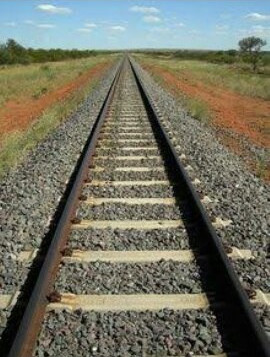
\includegraphics[height=3cm]{slike/railroad2.jpg}
	\end{center}
\end{frame}

\begin{frame}{Homogene koordinate - rješenje}
	\begin{itemize}
		\item $N$d koordinate prikazati sa $N+1$ brojem.
		\item Dodajemo novu koordinatu $w$
		\item $(x,y)$ postaje $(x,y,w)$
		\item $X = x/w$, $Y = y/w$
	\end{itemize}
	\begin{block}{Primjer}
		Točka $(1, 2)$ postaje u homogenim koordinatama $(1, 2, 1)$.
		
		Pomaknemo li tu istu točku beskonačno daleko: $(1, 2, 0)$. Odnosno, $(1/0, 2/0) = (\infty, \infty)$.
		
		Zaključno: možemo izraziti \textit{beskonačno} bez da napišemo znak $\infty$.
	\end{block}
\end{frame}

\begin{frame}{Sjecište dva paralelna pravca}
	\begin{align*}
		Ax + By + C &= 0 \\
		Ax + By + D &= 0
	\end{align*}
	Za $C \neq D$
	
	\begin{align*}
	A\frac{x}{w} + B\frac{y}{w} + C &= 0 \\
	A\frac{x}{w} + B\frac{y}{w} + D &= 0
	\end{align*}
	
	\begin{align*}
	Ax + By + Cw &= 0 \\
	Ax + By + Dw &= 0
	\end{align*}
	
	Rješenje: $(x, y, 0)$, jer je $(C-D)w=0$, $w=0$. Pravci se sijeku u točki na horizontu.
\end{frame}
\begin{frame}{Ipak je stvar malo kompliciranija}
	Osim što se homogene koordinate mogu shvatiti kao dobar trik za uniformni(homogeni) način primjene tranformacije, može se upotrijebiti i geometrijska interpretacija
	\\
	Jednostavno svakoj 2D točki dodajemo treću koordinatu, $w \neq 0$. Recimo da je to udaljenost od očišta.  Što je $w$ veći točka će se više će se pomaknuti.
\end{frame}


%\begin{frame}{Geometrijska interpretacija, 1d}
%	\[    \left[ \begin{array}{c}
%	x' \\ 1 \end{array} \right]  = \left[ \begin{array}{cc}
%	1 &  c \\
%	0 & 1 
%	\end{array} \right]  \left[ \begin{array}{c}
%	x \\ 1\end{array} \right]\]
%	
%	\begin{center}
%		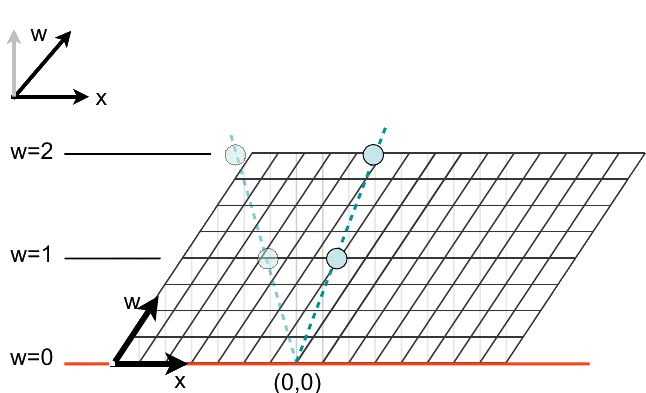
\includegraphics[width=5cm]{slike/translacija_1d_02.png}
%	\end{center}
%	Crvena linija i ishodište se ne pomiču $\rightarrow$ 2D smik.
%\end{frame}

\begin{frame}{Perspektivna ekvivalentnost}
	Svi umnošci skalara koji imaju vrijednost $\neq 0 $ se smatraju jednakim
	\begin{equation}
	\left[ \begin{array}{c}
	x \\ y \\ z\\ w\end{array} \right]  = 
	\left[ \begin{array}{c}
	ax \\ ay \\ az\\ aw\end{array} \right] = 
	\left[ \begin{array}{c}
	x/w \\ y/w \\ z/w\\ 1\end{array} \right] \nonumber
	\end{equation}
	za $ a\neq 0 $ i $ w\neq 0 $
	
	\begin{block}{Perspektiva}
		Sve 3D točke padaju na istu 2D koordinatu na slici.\\
		U tom smislu su sve takve 3D točke identične.
	\end{block}

\end{frame}

%\begin{frame}{Perspektivna ekvivalentnost - contd}
%	
%	\begin{block}{Perspektiva}
%		Sve 3D točke padaju na istu 2D koordinatu na slici.\\
%		U tom smislu su sve takve 3D točke identične.
%	\end{block}
%	\begin{center}
%		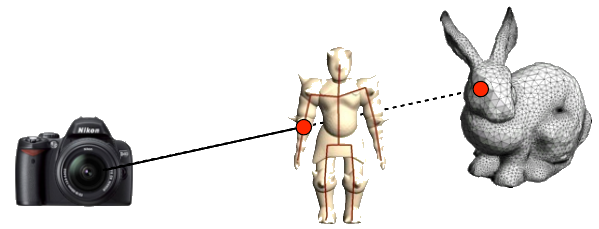
\includegraphics[width=6cm]{slike/homogenekoo_eqv.png}
%	\end{center}
%\end{frame}

\begin{frame}{1d primjer}
	1D točke $(x,w)$: Sve ekvivalentne homogene točke leže na linijama koje prolaze kroz ishodište koordinatnog sustava.
	\begin{center}
		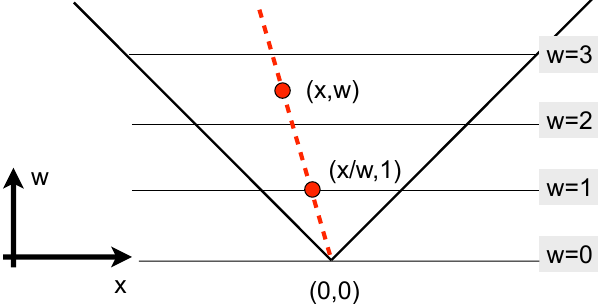
\includegraphics[height=4cm]{slike/homogenekoo_1d.png}
	\end{center}
\end{frame}

\begin{frame}{2d primjer}
	Potrebno samo podijeliti sa $w$
	\begin{center}
		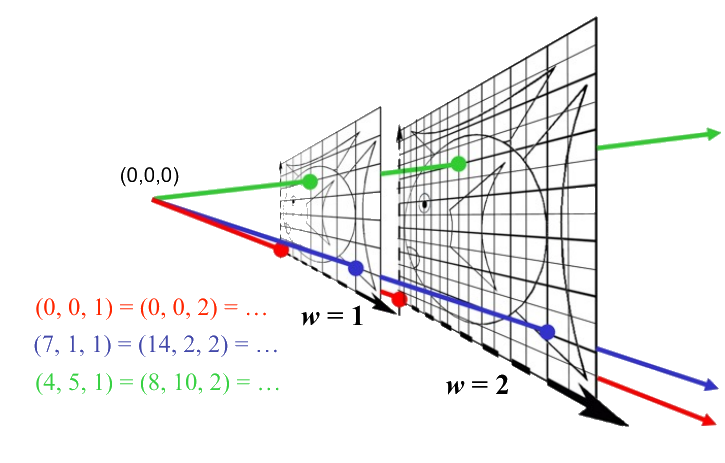
\includegraphics[width=10cm]{slike/homogenekoo_2d.png}
	\end{center}
\end{frame}


\begin{frame}{2d primjer, contd.}
	\only<1>{Kamera u ishodištu, pogled prema $z$ osi, $90\deg$, \textsl{image plane} na $z=1$}
	\only<2>{ Projicirana točka u homogenim koordinatama: 
		$$  p'=\left( \begin{array}{c}
		x/z \\
		1 \\
		1 
		\end{array} \right)$$}
	\only<3>{Ekvivalentno: \\$$ p'= \left( \begin{array}{c}
		x/z \\
		1 \\
		1 
		\end{array} \right) \propto  
		\left( \begin{array}{c}
		x \\
		z \\
		z 
		\end{array} \right)$$ }
	\begin{center}
		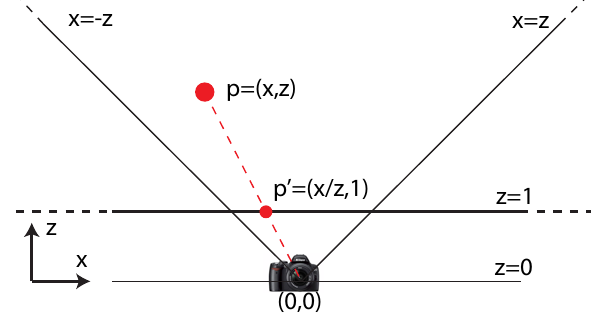
\includegraphics[width=7cm]{slike/perspective_2d.png}
	\end{center}
\end{frame}
\begin{frame}{Zaključno}
	\begin{itemize}
		\item Projekcijskim matricama dobijamo 2D projekciju 3D točaka.
		\item Kako se projicira na $z = 1$ ravninu,nestaje informacija o udaljenostima od očišta
		\begin{itemize}
			\item Potrebne udaljenosti za GPU tj. $Z$ međuspremnik, koji daje informaciju što je ispred ili iza čega
		\end{itemize}
	\end{itemize}	
\end{frame}



\section{2d transformacije}

\begin{frame}{2d transformacije i homogene koordinate }
	Transformacije će uvijek preslikavati točke u hiperravninu definiranu sa $w = 1$ na druge točke.
	Odnosno, transformacije $\mathbf{T}$ preslikavaju točku 
	$\mathbf{v} = \left[ \begin{array}{c} x \\ y \\ 1 \end{array} \right]$ u točku
	$\mathbf{v'} = \left[ \begin{array}{c} x' \\ y' \\ 1 \end{array} \right]$
	
	Linearne tranformacije koriste matricu oblika:
	\begin{equation}
	\mathbf{T} = 
	\left[ \begin{array}{ccc}
	a & b & 0\\
	d & e & 0 \\
	0 & 0 & 1 \end{array} \right] 
	\nonumber
	\end{equation}
	Afine: 
	\begin{equation}
	\mathbf{T} = 
	\left[ \begin{array}{ccc}
	a & b & c\\
	d & e & f \\
	0 & 0 & 1 \end{array} \right] 
	\nonumber
	\end{equation}
\end{frame}


\begin{frame}{Afine transformacije, homogene koordinate, receptura}
	\begin{itemize}
		\item Dodaje se jedna dimenzija više
		\begin{itemize}
			\item 2D: 3D vektor i 3x3 matrice
			%			\item 3D: 4D vektor i 4x4 matrice
			\item Afine transformacije postaju linearne u višoj dimenziji
		\end{itemize}
		\item Svaka točka ima dodatnu vrijednost, $w=1$		
	\end{itemize}
\end{frame}


%\begin{frame}{2d primjer}
%$w=0$? Točka na beskonačno daleko
%\begin{center}
%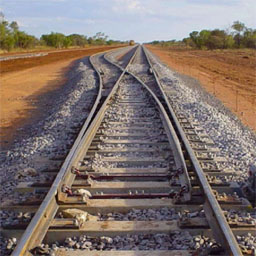
\includegraphics[height=1cm]{slike/railroad.jpg}
%\end{center}
%\begin{center}
%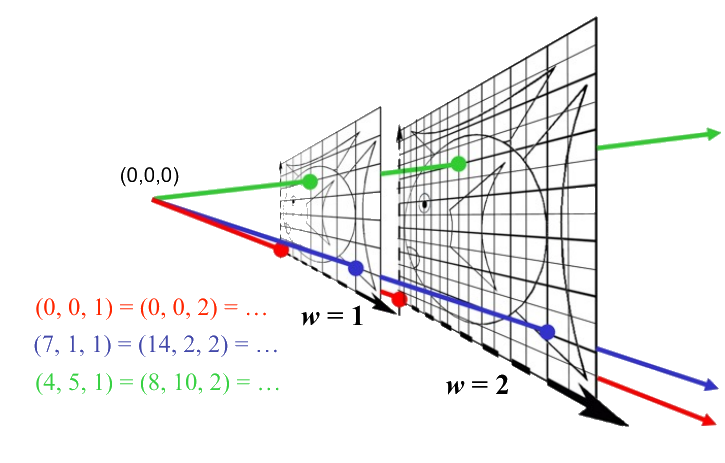
\includegraphics[width=7cm]{slike/homogenekoo_2d.png}
%\end{center}
%\end{frame}



%\begin{frame}{Translacije i homogene koordinate}
%	Dodajemo novu dimenziju jer translacija postaje linearna transformacija u višoj dimenziji. \\
%	Odnosno, translacija se može prikazati matrično
% \[    \left[ \begin{array}{c}
%                 x' \\ y' \\ z' \\ 1\end{array} \right]  = \left[ \begin{array}{cccc}
%                1 & 0 & 0 & t_{x} \\
%		0 & 1 & 0 & t_{y} \\
%		0 & 0 & 1 & t_{z} \\
%		0 & 0 & 0 & 1 
%         \end{array} \right]  \left[ \begin{array}{c}
%                          x \\ y \\ z \\ 1\end{array} \right]\]
%\end{frame}


% % % % % % % % % % % % % % % % % % % % % % % % % % % % % % % % % % % % % % % % % % % % % %

\begin{frame}{Translacija}
	\begin{center}
		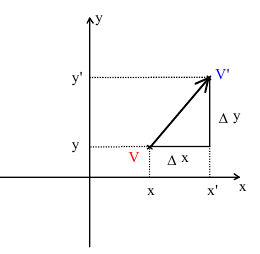
\includegraphics[height=3cm]{slike/2dtranslacija.png}
	\end{center}
	Matrica transformacije ima oblik: :
	\begin{equation}
	\mathbf{T} = 
	\left[ \begin{array}{ccc}
	1 & 0 & dx\\
	0 & 1 & dy \\
	0 & 0 & 1 \end{array} \right] 
	\nonumber
	\end{equation}
	odnosno:
	\begin{equation}
	\mathbf{Tv} = 
	\left[ \begin{array}{ccc}
	1 & 0 & dx\\
	0 & 1 & dy \\
	0 & 0 & 1 \end{array} \right] 
	\left[ \begin{array}{c}
	x\\
	y \\
	1 \end{array} \right] = 
	\left[ \begin{array}{c}
	x+dx\\
	y+dy \\
	1 \end{array} \right] = \mathbf{v'}
	\nonumber
	\end{equation}
\end{frame}


\begin{frame}{Rotacija - oko ishodišta}
	\begin{center}
		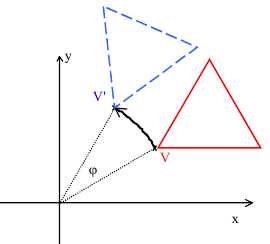
\includegraphics[height=3.5cm]{slike/2drotacija.png}
	\end{center}
	$$ \begin{array}{cc} x' = x \text{cos}(\phi)-y\text{sin}(\phi)  & 
	y' = x \text{sin}(\phi)+y\text{cos}(\phi) \end{array}$$
	$$ \left[ \begin{array}{c} x' \\ y' \\ h'  \end{array} \right] = 
	\left[ \begin{array}{ccc}
	\text{cos}(\phi) & -\text{sin}(\phi) & 0 \\
	\text{sin}(\phi) & \text{cos}(\phi) & 0 \\
	0 & 0 & 1 
	\end{array} \right]\left[ \begin{array}{c} x \\ y \\ h \end{array} \right] 
	\rightarrow \mathbf{V'} =  \mathbf{R}\mathbf{V} $$
	
\end{frame}

\begin{frame}{Skaliranje}
	\begin{center}
		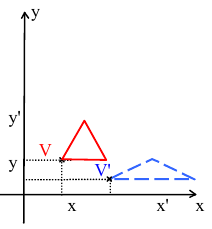
\includegraphics[height=2cm]{slike/2dskaliranje.png}
	\end{center}
	$$ \begin{array}{cc} x' = x s_{x}  & 
	y' = y s_{y} \end{array}$$
	$$ \left[ \begin{array}{ccc} x' & y' & h'  \end{array} \right] = 
	\left[ \begin{array}{ccc} x & y & h \end{array} \right] 
	\left[ \begin{array}{ccc}
	s_{x} & 0 & 0 \\
	0 & s_{y} & 0 \\
	0 & 0 & 1 
	\end{array} \right] \rightarrow \mathbf{V'} = \mathbf{V} \mathbf{S} $$
	Negativan $s_{x}$ daje zrcaljenje oko koo. osi $x$, analogno za $s_{y}$
	\[ \left[ \begin{array}{ccc}
	s & 0 & 0 \\
	0 & s & 0 \\
	0 & 0 & 1 
	\end{array} \right] = 
	\left[ \begin{array}{ccc}
	1 & 0 & 0 \\
	0 & 1 & 0 \\
	0 & 0 & 1/s 
	\end{array} \right]\]
	
\end{frame}

\begin{frame}{Smik}
	\begin{center}
		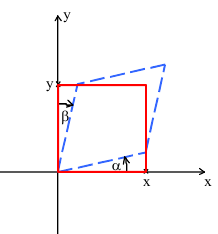
\includegraphics[height=3.5cm]{slike/2dsmik.png}
	\end{center}
	$$ \begin{array}{cc} x' = x+y\text{tan}(\beta)  & 
	y' = y+x\text{tan}(\alpha) \end{array}$$
	$$ \left[ \begin{array}{c} x' \\ y' \\ h'  \end{array} \right] = 
	\left[ \begin{array}{ccc}
	1 & \text{tan}(\beta) & 0 \\
	\text{tan}(\alpha) & 1 & 0 \\
	0 & 0 & 1 
	\end{array} \right]
	\left[ \begin{array}{c} x \\ y \\ h \end{array} \right] 
	$$
	
\end{frame}

\begin{frame}{Inverzne transformacije}
	Traženje inverza matrice:
	Translacija
	\[ \left[ \begin{array}{ccc}
	1 & 0 & 0 \\
	0 & 1 & 0 \\
	t_{x} & t_{y} & 1 
	\end{array} \right] ^{-1}  =  \left[ \begin{array}{ccc}
	1 & 0 & 0 \\
	0 & 1 & 0 \\
	-t_{x} & -t_{y} & 1 
	\end{array} \right] \]
	Skaliranje
	\[ \left[ \begin{array}{ccc}
	s_{x} & 0 & 0 \\
	0 & s_{y} & 0 \\
	0 & 0 & 1 
	\end{array} \right]^{1} = 
	\left[ \begin{array}{ccc}
	1/s_{x} & 0 & 0 \\
	0 & 1/s_{y} & 0 \\
	0 & 0 & 1 
	\end{array} \right]\]
\end{frame}

\begin{frame}{Inverzne transformacije contd.}
	Rotacija
	\[  \left[ \begin{array}{ccc}
	\text{cos}(\phi) & \text{sin}(\phi) & 0 \\
	-\text{sin}(\phi) & \text{cos}(\phi) & 0 \\
	0 & 0 & 1 
	\end{array} \right] ^{-1} = 
	\left[ \begin{array}{ccc}
	\text{cos}(\phi) & -\text{sin}(\phi) & 0 \\
	\text{sin}(\phi) & \text{cos}(\phi) & 0 \\
	0 & 0 & 1 
	\end{array} \right]\]
	\begin{block}{Bitno}
		Inverzna matrica ortogonalne matrice je njena transponirana matrica
	\end{block}
\end{frame}

\begin{frame}{Važno}
	\[ \left[ \begin{array}{ccc} x' & y' & h'  \end{array} \right] = 
	\left[ \begin{array}{ccc} x & y & h \end{array} \right] 
	\left[ \begin{array}{ccc}
	1 & 0 & 0 \\
	0 & 1 & 0 \\
	t_{x} & t_{y} & 1 
	\end{array} \right]  \]
	\[ \left[ \begin{array}{c} x' \\ y' \\ h'  \end{array} \right] =     
	\left[ \begin{array}{ccc}
	1 & 0 & t_{x} \\
	0 & 1 & t_{y} \\
	0 & 0 & 1 
	\end{array} \right]
	\left[ \begin{array}{c} x \\ y \\ h \end{array} \right] 
	\]
\end{frame}

\section{3D transformacije}
\begin{frame}{Translacija}
	\begin{block}{Translacijska matrica}
		\[    \mathbf{T}_{T} = \left[ \begin{array}{cccc}
		1 & 0 & 0 & t_{x} \\
		0 & 1 & 0 & t_{y} \\
		0 & 0 & 1 & t_{z} \\
		0 & 0 & 0 & 1 
		\end{array} \right] \]
	\end{block}
\end{frame}
\begin{frame}{Translacija}
	\begin{block}{Primjer}
		\[    \left[ \begin{array}{c}
		x' \\ y' \\ z'\\ w'
		\end{array} \right] =  
		\left[ \begin{array}{cccc}
		1 & 0 & 0 & t_{x} \\
		0 & 1 & 0 & t_{y} \\
		0 & 0 & 1 & t_{z} \\
		0 & 0 & 0 & 1 
		\end{array} \right] \cdotp 
		\left[ \begin{array}{c}
		x \\ y \\ z\\ 1
		\end{array} \right]\]
		Postavi li se $ w_{h} = 1 $
		\[	x'= x+t_{x} \]
		\[	y'= y+t_{y} \]
		\[	z'= z+t_{z} \]
	\end{block}
\end{frame}

\begin{frame}{Skaliranje}
	\begin{block}{Tranformacijska matrica }
		\[    \mathbf{T}_{S} = \left[ \begin{array}{cccc}
		s_{x} & 0 & 0 & 0 \\
		0 & s_{y} & 0 & 0 \\
		0 & 0 & s_{z} & 0 \\
		0 & 0 & 0 & 1 
		\end{array} \right] \]
	\end{block}
\end{frame}

\begin{frame}{Rotacija}
	\begin{block}{Rotacija oko $x$ osi}
		\[    \mathbf{T}_{R_{x}} = \left[ \begin{array}{cccc}
		1 & 0 & 0 & 0 \\
		0 & \mathtt{cos}\theta & -\mathtt{sin}\theta & 0 \\
		0 & \mathtt{sin}\theta & \mathtt{cos}\theta & 0 \\
		0 & 0 & 0 & 1 
		\end{array} \right] \]
	\end{block}
\end{frame}

\begin{frame}{Rotacija contd.}
	\begin{block}{Rotacija oko $y$ osi}
		\[    \mathbf{T}_{R_{y}} = \left[ \begin{array}{cccc}
		\mathtt{cos}\theta & 0 & \mathtt{sin}\theta & 0 \\
		0 & 1 & 0 & 0 \\
		-\mathtt{sin}\theta & 0 & \mathtt{cos}\theta & 0 \\
		0 & 0 & 0 & 1 
		\end{array} \right] \]
	\end{block}
\end{frame}

\begin{frame}{Rotacija contd.}
	\begin{block}{Rotacija oko $z$ osi}
		\[    \mathbf{T}_{R_{z}} = \left[ \begin{array}{cccc}
		\mathtt{cos}\theta & -\mathtt{sin}\theta & 0 & 0 \\
		\mathtt{sin}\theta & \mathtt{cos}\theta & 0 & 0 \\
		0 & 0 & 1 & 0 \\
		0 & 0 & 0 & 1 
		\end{array} \right] \]
	\end{block}
\end{frame}


\begin{frame}{Transformacija - Preslikavanje}
	Preslikavanje iz jednog u drugi koordinatni sustav\\
	Npr. x-y-z u x'-y'-z'.
	$$ x'\rightarrow \left(\theta_{x'x}, \theta_{x'y}, \theta_{x'z}\right)$$
	$$ y'\rightarrow \left(\theta_{y'x}, \theta_{y'y}, \theta_{y'z}\right)$$
	$$ z'\rightarrow \left(\theta_{z'x}, \theta_{z'y}, \theta_{z'z}\right)$$
\end{frame}

\begin{frame}{Transformacija - Preslikavanje}
	\begin{block}{Preslikavanje}
		\[    \mathbf{T}_{R} = \left[ \begin{array}{cccc}
		\mathtt{cos}\theta_{x'x} & \mathtt{cos}\theta_{x'y} & \mathtt{cos}\theta_{x'z} & 0 \\
		\mathtt{cos}\theta_{y'x} & \mathtt{cos}\theta_{y'y} & \mathtt{cos}\theta_{y'z} & 0 \\
		\mathtt{cos}\theta_{z'x} & \mathtt{cos}\theta_{z'y} & \mathtt{cos}\theta_{z'z} & 0 \\
		0 & 0 & 0 & 1 
		\end{array} \right] \]
	\end{block}
\end{frame}

\section{Složene transformacije}
\begin{frame}{Složene transformacije}
	Skaliranje i translacija:
	\begin{center}
		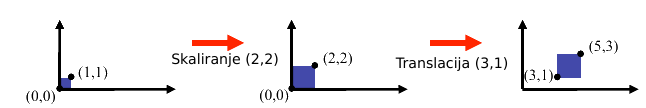
\includegraphics[width=10cm]{slike/slozene_transformacije_01.png}
	\end{center}
	$$ TS = \left[ \begin{array}{ccc}
	1 & 0 & 3 \\
	0 & 1 & 1  \\
	0 & 0 & 1 
	\end{array} \right]
	\left[ \begin{array}{ccc}
	2 & 0 & 0 \\
	0 & 2 & 0  \\
	0 & 0 & 1 
	\end{array} \right] = 
	\left[ \begin{array}{ccc}
	2 & 0 & 3 \\
	0 & 2 & 1  \\
	0 & 0 & 1 
	\end{array} \right]
	$$
\end{frame}

\begin{frame}{Složene transformacije - contd.}
	Skaliranje i translacija - $p' = T(Sp) = TS p$:
	\begin{center}
		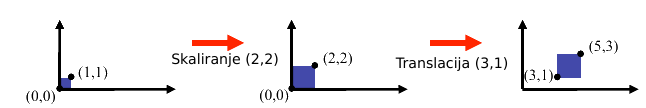
\includegraphics[width=10cm]{slike/slozene_transformacije_01.png}
	\end{center}
	Translacija i skaliranje - $p' = S(Tp) = ST p$:
	\begin{center}
		
\includegraphics[width=10cm]{slike/slozene_transformacije_02.png}
	\end{center}
\end{frame}

\begin{frame}{Složene transformacije - contd.}
	Skaliranje i translacija - $p' = T(Sp) = TS p$:
	$$ TS = \left[ \begin{array}{ccc}
	1 & 0 & 3 \\
	0 & 1 & 1  \\
	0 & 0 & 1 
	\end{array} \right]
	\left[ \begin{array}{ccc}
	2 & 0 & 0 \\
	0 & 2 & 0  \\
	0 & 0 & 1 
	\end{array} \right] = 
	\left[ \begin{array}{ccc}
	2 & 0 & 3 \\
	0 & 2 & 1  \\
	0 & 0 & 1 
	\end{array} \right]
	$$
	Translacija i skaliranje - $p' = S(Tp) = ST p$:
	$$ TS = \left[ \begin{array}{ccc}
	2 & 0 & 0 \\
	0 & 2 & 0  \\
	0 & 0 & 1 
	\end{array} \right]
	\left[ \begin{array}{ccc}
	1 & 0 & 3 \\
	0 & 1 & 1  \\
	0 & 0 & 1 
	\end{array} \right] = 
	\left[ \begin{array}{ccc}
	2 & 0 & 6 \\
	0 & 2 &2  \\
	0 & 0 & 1 
	\end{array} \right]
	$$
\end{frame}

\begin{frame}{Složene transformacije}
	\[ \left[ \begin{array}{c}
	x' \\ y' \\ z'\\ w'
	\end{array}   \right]   = \]  
	\[ \left( \left[ \begin{array}{cccc}
	1 & 0 & 0 & t_{x} \\
	0 & 1 & 0 & t_{y} \\
	0 & 0 & 1 & t_{z} \\
	0 & 0 & 0 & 1 
	\end{array} \right] 
	\left[ \begin{array}{cccc}
	\mathtt{cos}\theta & 0 & \mathtt{sin}\theta & 0 \\
	0 & 1 & 0 & 0 \\
	-\mathtt{sin}\theta & 0 & \mathtt{cos}\theta & 0 \\
	0 & 0 & 0 & 1 
	\end{array} \right] 
	\left[ \begin{array}{cccc}
	s_{x} & 0 & 0 & 0 \\
	0 & s_{y} & 0 & 0 \\
	0 & 0 & s_{z} & 0 \\
	0 & 0 & 0 & 1 
	\end{array} \right] \right)
	\left[ \begin{array}{c}
	x \\ y \\ z\\ w
	\end{array}   \right] \]
	\[ \mathbf{p}' = \left(\mathbf{T}_T \mathbf{T}_{R_{y}} \mathbf{T}_{S} \right)\mathbf{p} \]
\end{frame}

\begin{frame}
	Malo o množenju\\
	\[ \mathbf{p}' = \left(\mathbf{T}_T \mathbf{T}_{R_{y}} \mathbf{T}_{S} \right)\mathbf{p} \]
	\[ \mathbf{p}' = \left( \mathbf{T}_T \left( \mathbf{T}_{R_{y}} 
	\left( \mathbf{T}_{S} \mathbf{p} \right) \right) \right) \]
	\alert{ \[ \mathbf{p}' = \mathbf{T}_T \mathbf{T}_{R_{y}} \mathbf{T}_{S}\mathbf{p} \] }
	Odnosno: \Large{Redoslijed operacija je BITAN!}
\end{frame}

%\begin{frame}{Rotacija oko proizvoljnog vektora}
%
%\end{frame}
\begin{frame}{Inverzne transformacije}
	\begin{itemize}
		\item<1-> translacija - inverzna matrice translacije odgovara inverznoj 
		transformaciji tj. pomaku u suprotnom smjeru, odnosno mijenja se
		\textbf{predznak pomaka} duž pojedinih osi
		\item<2-> rotacija – inverzna matrice rotacije odgovara inverznoj
		transformaciji tj. transponiranoj matrici originalne rotacije, jednostavnije, rotaciji u suprotnom smjeru, odnosno mijenja se \textbf{predznak kuta} rotacije
		\item<3-> skaliranje - inverzna matrice skaliranja odgovara inverznoj
		transformaciji tj. povećavanje odgovara smanjivanju, odnosno
		mijenja se faktor skaliranja u \textbf{recipročnu} vrijednost
	\end{itemize}
\end{frame}

\section{Transformacija normala}
\begin{frame}{Problem}
	
	Zadane su točke $T_1(0,0)$ i $T_2(5,1)$. Vektor pravca je $\vec{v} = T_2 - T_1 = (5,1)$
	
	Normala vektora $\vec{v}$: $\vec{n} = (-1, 5)$, jer je $\vec{v}\cdot\vec{n}=0$
	
	Zadajmo transformaciju: $$\mathbf{M} = \left[\begin{array}{ccc}
	1 & 0& 0 \\
	0 & 2 & 0 \\
	0 & 0 & 1
	\end{array}\right]$$
	
	Nove točke su $T'_1 = \mathbf{M}T_1 = (0,0)$ i $T'_2 = \mathbf{M}T_2=(5, 2)$
	
	Vektor pravca je sada $\vec{v}' = T'_2 - T'_1 = (5,2)$ 
	
	Skalirana normala je $\vec{n}' = \mathbf{M}\vec{n} = (-1, 10)$
	
	Sada $\vec{v}\cdot'\vec{n}'\neq0$
\end{frame}

\begin{frame}{Rješenje}
	Treba matrično množiti - ovdje su vektori napisani kao jedan redak:
	\onslide<+->{
		$$\mathbf{v} \mathbf{n}^T = 0$$}
	\onslide<+->{
		Vektor $\mathbf{v}$ množimo sa $\mathbf{M}$, tada nam skalarni produkt ne vrijedi. Zato moramo \textit{poništiti} operaciju s inverznom matricom transformacije, da dobijemo jediničnu matricu $\mathbf{I}$:
		$$\mathbf{v} \mathbf{M}\mathbf{M}^{-1}\mathbf{n}^T = 0$$}
	
	\onslide<+->{
		Grupiramo operacije: 
		$$(\mathbf{v} \mathbf{M})(\mathbf{M}^{-1}\mathbf{n}^T) = 0$$
	}
\end{frame}
\begin{frame}{Rješenje, contd.}
	$$(\mathbf{v} \mathbf{M})(\mathbf{M}^{-1}\mathbf{n}^T) =\mathbf{v}'\mathbf{n}'^{T} =0$$
	
	\onslide<+->{$\mathbf{n}'^{T} = \mathbf{M}^{-1}\mathbf{n}^T$ }
	
	\onslide<+->{$\mathbf{n}' = (\mathbf{M}^{-1}\mathbf{n}^T)^T$ }
	
	\onslide<+->{Na kraju: $\mathbf{n}' = \mathbf{n}{\mathbf{M}^{-1}}^T$ 
		
		Normala se dobije množenjem \textbf{inverzne transponirane} matrice transformacije.
	}
	
	\onslide<+->{
		Za naš primjer: 
		
		$\mathbf{M}^{-1} = \left[\begin{array}{ccc}
		1 & 0& 0 \\
		0 & 1/2 & 0 \\
		0 & 0 & 1
		\end{array}\right]$, i 
		${\mathbf{M}^{-1}}^T = \left[\begin{array}{ccc}
		1 & 0& 0 \\
		0 & 1/2 & 0 \\
		0 & 0 & 1
		\end{array}\right]$
	}
\end{frame}
\plain{Pitanja?}
\end{document}